\documentclass[conference]{IEEEtran}
\IEEEoverridecommandlockouts
% The preceding line is only needed to identify funding in the first footnote. If that is unneeded, please comment it out.
\usepackage{cite}
\usepackage[ngerman]{babel}
\usepackage[utf8]{inputenc}
\usepackage{amsmath,amssymb,amsfonts}
\usepackage{algorithmic}
\usepackage{graphicx}
\usepackage{textcomp}
\usepackage{xcolor}
\usepackage{listings}


\definecolor{pblue}{rgb}{0.13,0.13,1}
\definecolor{pgreen}{rgb}{0,0.5,0}
\definecolor{pred}{rgb}{0.9,0,0}
\definecolor{pgrey}{rgb}{0.46,0.45,0.48}
\lstset{language=Java,
	showspaces=false,
	showtabs=false,
	breaklines=true,
	tabsize=2,
	showstringspaces=false,
	breakatwhitespace=true,
	commentstyle=\color{pgreen},
	keywordstyle=\color{pblue},
	stringstyle=\color{pred},
	basicstyle=\ttfamily
}


\usepackage{url}
\def\BibTeX{{\rm B\kern-.05em{\sc i\kern-.025em b}\kern-.08em
		T\kern-.1667em\lower.7ex\hbox{E}\kern-.125emX}}
\begin{document}
	
	\title{Computational Geometry - Abgabe 2}
	
	\author{\IEEEauthorblockN{1\textsuperscript{st} Bartolovic Eduard}
		\IEEEauthorblockA{\textit{Hochschule München} \\
			München, Deutschland \\
			eduard.bartolovic0@hm.edu}
	}
	
	\maketitle
	
	\begin{abstract}
		
		
	\end{abstract}
	
	\section{Berechnung des Flächeninhalts von einem Dreieck}
	Für die Berechnung der Fläche eines Dreiecks wird die Formel verwendet:
	\[ A = \frac{1}{2} ccw(p_1,p_2,p_3) \]
	Der CCW ist so definiert: 
	\[ ccw(p,q,r) := 
	\begin{vmatrix}
		p_1 & p_2 & 1 \\ 
		q_1 & q_2 & 1 \\ 
		r_1 & r_2 & 1 \notag
	\end{vmatrix} \]
	
	\section{Berechnung der Fläche eines Polygons}
	Für die Berechnung der Fläche eines Polygons berechnet man die Summe aller Flächen der Dreiecke die sich mit den Eckpunkten des Polygons und dem Nullpunkt bilden lassen können.
	\begin{figure}[h]
		\begin{center}
			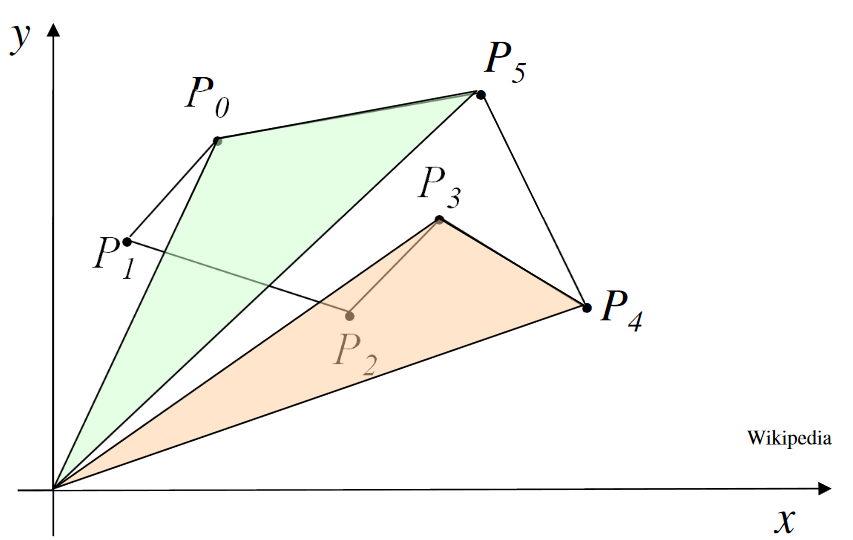
\includegraphics[width=6cm]{AreaPoly.png}
			\caption{Berechnung der Fläche eines Polygons mit mehreren Dreiecken}
			\label{figure_3}
		\end{center}
	\end{figure}
	\[ A = \sum_{i=1}^{n} \frac{ccw(0,p_n,p_{n+1})}{2} \]
	Da in die Formel des ccw der Nullpunkt eingesetzt wird lässt sich das Problem vereinfachen:
	\[ ccw(p,q,r) = p_x*q_y - p_y*q_x + q_x*r_y - q_y*r_x + p_y*r_x - p_x*r_y \]
	\[ ccw(0,q,r) = 0*q_y - p_y*q_x + q_x*r_y - q_y*r_x + 0*r_x - 0*r_y \]
	\[ ccw(0,q,r) = 0*q_y - 0*q_x + q_x*r_y - q_y*r_x + 0*r_x - 0*r_y \]
	\[ ccw(0,q,r) =  q_x*r_y - q_y*r_x  \]
	Zurück in die Formel eingesetzt:
	\[ A = \sum_{i=1}^{n} \frac{(x_{i}*y_{i+1}-y_{i}*x_{i+1})}{2}\]
	Um die Anzahl der Divisionen zu verringern wird das $\frac{1}{2}$ aus der Summe herausgezogen:
	\[ A= \frac{1}{2}\sum_{i=1}^{n}(x_{i}*y_{i+1}-y_{i}*x_{i+1})\]
	Zusätzlich lässt sich auch noch die Anzahl der Multiplikationen verringern \cite{b1}:
	\[ A = \frac{1}{2}\sum_{i=1}^{n}(x_{i}*y_{i+1}-y_{i}*x_{i+1})\]	
	\[ = \frac{1}{2}\sum_{i=1}^{n}(x_{i}*y_{i+1}) - \frac{1}{2}\sum_{i=1}^{n}(y_{i}*x_{i+1})\]	
	\[ = \frac{1}{2}\sum_{i=2}^{n+1}(x_{i-1}*y_{i}) - \frac{1}{2}\sum_{i=1}^{n}(y_{i}*x_{i+1})\]
	\[ = \frac{1}{2} \underbrace{\sum_{i=2}^{n+1}(x_{i-1}*y_i)}_{\substack{ = \sum_{i=1}^{n}(x_{i-1}*y_{i})  \text{, da } y_{n+1}=y_i \text{ und } x_0=x_n}} - \frac{1}{2}\sum_{i=1}^{n}(y_i*x_{i+1})\]
	\[ = \frac{1}{2} \sum_{i=1}^{n}(x_{i-1}*y_{i}) - \frac{1}{2}\sum_{i=1}^{n}(y_i*x_{i+1})\]
	\[ = \frac{1}{2}\sum_{i=1}^{n}(x_{i-1}*y_{i}-y_{i}*x_{i+1})\]
	\[ A= \frac{1}{2}\sum_{i=1}^{n} y_i(x_{i-1}-x_{i+1})\]
	Wenn die Eckpunkte gegen den Uhrzeigersinn definiert sind dann ist die Fläche positiv. Im Uhrzeigersinn ist die Fläche negativ.
	
	
	\section{Berechnung der Fläche eines Bundeslandes}
	Ein Bundesland besteht mindestens aus einem Polygon. Manche Bundesländer sind aber über mehrere Polygone definiert. So zum Beispiel besitzt Niedersachsen Inseln die einzeln definiert sind. Auch ist die Stadt Bremen als Loch definiert. 
	\begin{figure}[h]
		\begin{center}
			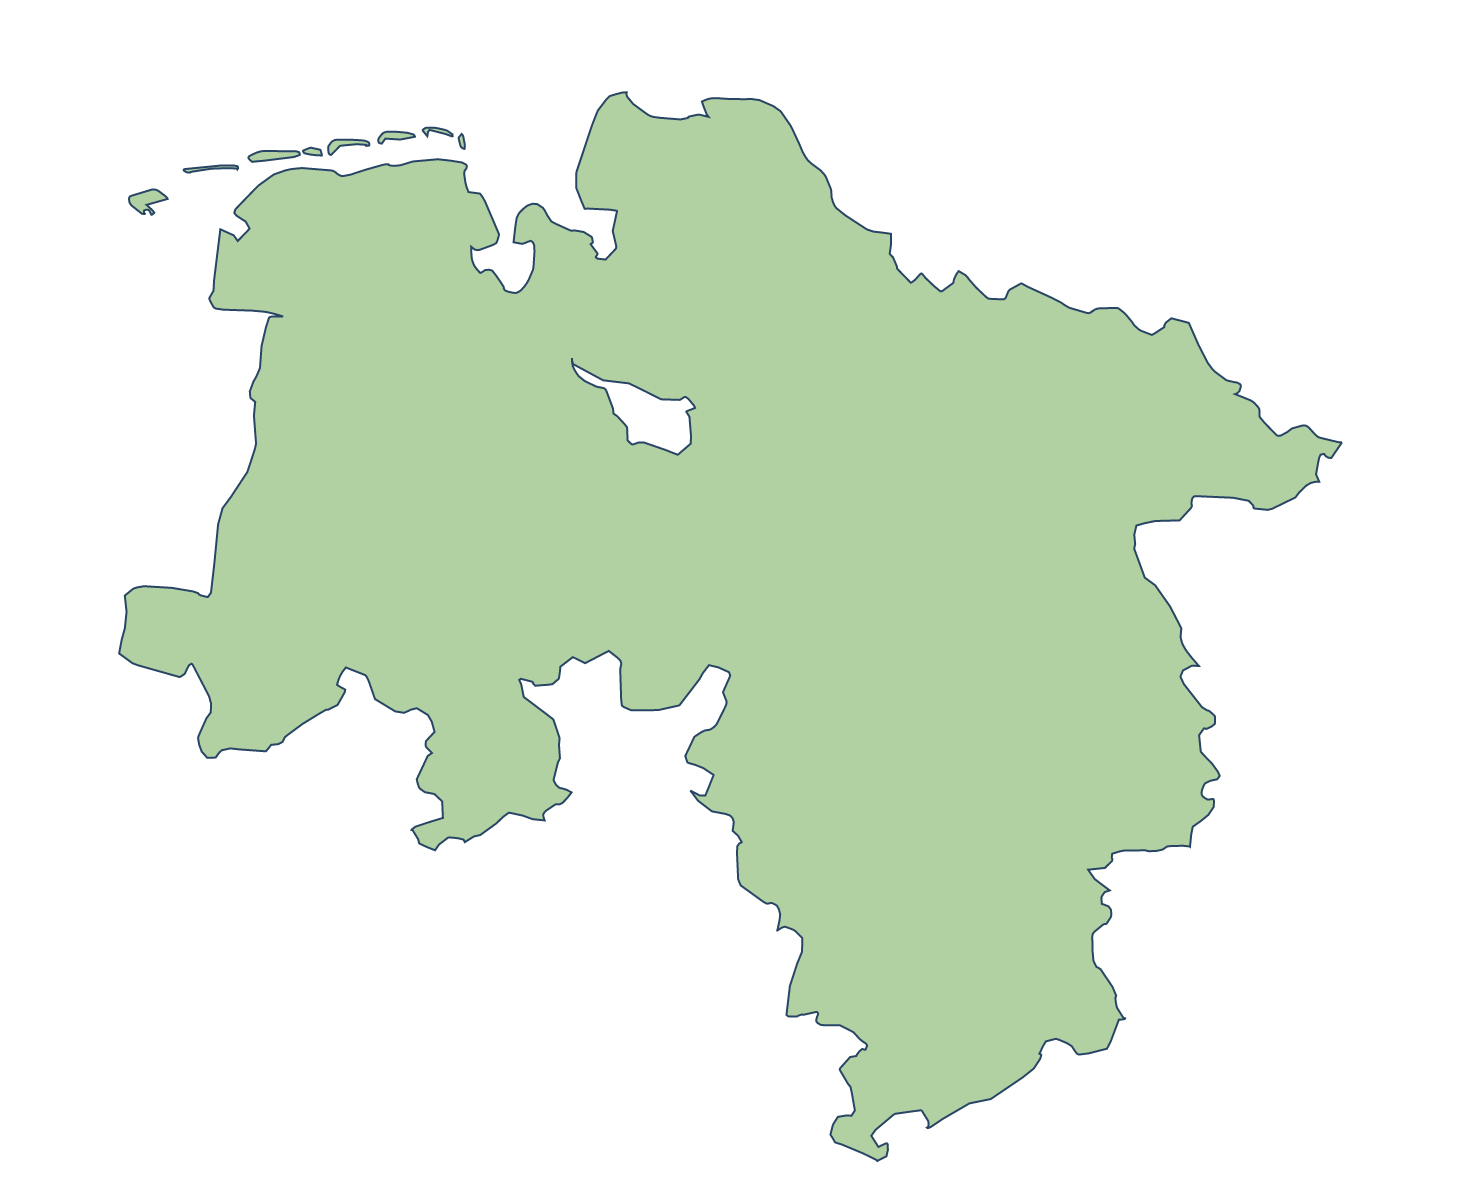
\includegraphics[width=8cm]{Niedersachsen.png}
			\caption{Niedersachsen}
			\label{Niedersachsen}
		\end{center}
	\end{figure}\\
	So muss die Fläche der Inseln und der Hauptfläche summiert werden. Die Fläche der Stadt Bremen aber abgezogen werden. Idealerweise hätte das Loch ein negatives Vorzeichen und die Inseln alle ein positives Vorzeichen sodass einfach eine Summe über alle Polygone gebildet werden kann.\\
	Das Problem mit dem vorliegenden Datensatz ist das dieser sich nicht an die Konvention bezüglich des Vorzeichens der Fläche und der Definierung der Eckpunkte im Uhrzeigersinn hält. So gibt es Inseln die eine negative Fläche besitzen oder Löcher mit postivem Vorzeichen.\\
	Aus diesem Grund werden erst einmal alle positiv Flächen behandelt. Zusätzlich muss eine neue Überprüfung stattfinden die überprüft ob ein Polygon ein Loch ist. Hierbei wird getestet ob ein Polygon in einem anderen Polygon vollständig enthalten ist.
	\subsection{Sonderfall: Polygon in einem anderen Polygon}
	Wie testet man ob ein Polygon $P_{klein}$ in einem anderen Polygon $P_{groß}$ vollständig enthalten ist?
	Ein einfacher Ansatz ist es zu überprüfen ob sich alle Punkte des Polygons $P_{klein}$ in $P_{groß}$ befinden.\\
	Dies würde für die Aufgabe bei der Flächenberechnung der Bundesländer schon funktionieren.\\
	Es gebe nur einen Sonderfall wie den in der Abbildung \ref{polyInPoly}. Mit dem oben beschriebenen Ansatz würde $P_{klein}$ trotzdem als Loch bezeichnet werden da alle Eckpunkte von $P_{klein}$ in $P_{groß}$ befinden.
	\begin{figure}[h]
		\begin{center}
			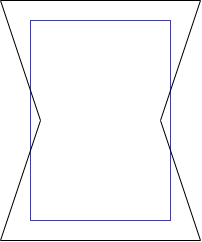
\includegraphics[width=4cm]{PolyInPoly.png}
			\caption{Ein Randfall in dem das blaue Polygon nicht im schwarzen liegt}
			\label{polyInPoly}
		\end{center}
	\end{figure}\\
	Jetzt könnte man zusätzlich überprüfen ob sich alle Punkte von $P_{groß}$ außerhalb von $P_{klein}$ befinden. Doch dies würde auch noch nicht alle Probleme wie man in Abbildung \ref{polyInPoly2} sehen kann lösen.
	\begin{figure}[h]
		\begin{center}
			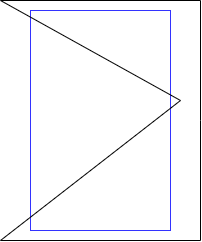
\includegraphics[width=4cm]{PolyInPoly2.png}
			\caption{Ein Randfall in dem das blaue Polygon nicht im schwarzen liegt}
			\label{polyInPoly2}
		\end{center}
	\end{figure}\\
	Deshalb müsste man alle Kanten $P_{groß}$ und $P_{klein}$ nach Schnittpunkten untersuchen.
	
	\section{Überprüfung ob ein Punkt in einem Polygon liegt}
	Für die Überprüfung ob ein Punkt $\tilde{p}$ in einem Polygon P liegt wird zuerst Strecke aus dem Punkt $\tilde{p}$ zu einem festgelegtem Punkt $\tilde{q}$ definiert. Der Punkt $\tilde{q}$ muss außerhalb des Polygons P liegen. Dabei legt man den Punkt rechts vom Polygon P und auf der selben Höhe des Punktes $\tilde{p}$.\\
	Um sicher zu gehen das sich ein Punkt rechts von einem Polygon P befindet, iteriert man über alle Eckpunkte des Polygons und sucht dabei den höchsten X Wert und addiert dann einen Faktor darauf.\\
	Jetzt zählt man die Schnittpunkte nur mit echten Seitenwechseln zwischen der Strecke $[\tilde{p}\tilde{q}]$ und allen Kanten des Polygons P. Dabei startet man bei einem Eckpunkt $p_{Start}$ der nicht auf $[\tilde{p}\tilde{q}]$ liegt. Ist die Anzahl ungerade liegt der Punkt p im Polygon P. Ist die Anzahl gerade liegt p außerhalb von P.\\
	Um echte Seitenwechsel zu identifizieren wird muss folgende Bedingung wahr sein:
	\[ ccw(p_{i-1} , p_i, \tilde{p}) * ccw(p_{i-1} , p_i, \tilde{q}) \leq 0 \]
	Zusätzlich muss der Fall abgedeckt werden das der Punkt p auf der Kante des Polygons liegt. Hierbei iteriert man einfach über alle Kanten $[p_n,q_n]$.\\
	Die Abbildung \ref{PointInPoly} zeigt die wichtigsten Fälle die abgedeckt werden müssen.
	\begin{figure}[h]
		\begin{center}
			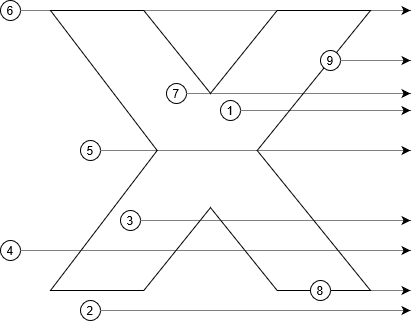
\includegraphics[width=8cm]{PointInPolygon.png}
			\caption{Verschiedene Fälle wie ein Punkt in einem Polygon liegen kann.}
			\label{PointInPoly}
		\end{center}
	\end{figure}\\
	In folgender Tabelle werden die einzelnen Punkte/Fälle kurz beschrieben. So wird die Anzahl der Schnittpunkte, die Anzahl der echten Seitenwechsel und der Output des Algorithmus aufgelistet.\\
	
	\scalebox{0.9}{
	\begin{tabular}{|c|c|c|c|c|}
		\hline
		\textbf{Punkt} & \textbf{Schnittpunkte} & \textbf{Seitenwechsel} & \textbf{Kante} & \textbf{Output} \\
		\hline
		1 & 1 & 1 & Nein & Inside \\
		\hline
		2 & 0 & 0 & Nein & Outside \\
		\hline
		3 & 3 & 3 & Nein & Inside \\
		\hline
		4 & 4 & 4 & Nein & Outside \\
		\hline
		5 & 2 & 2 & Nein & Outside \\
		\hline
		6 & $\infty$ & 0 & Nein & Outside \\
		\hline
		7 & 2 & 1 & Nein & Inside \\
		\hline
		8 & $\infty$ & 0 & Ja & Inside \\
		\hline
		9 & 1 & 0 & Ja & Inside \\
		\hline
	\end{tabular}
	}
	\vspace{1cm}
	\section{Überprüfung ob eine Stadt in einem Bundesland liegt}
	Um zu überprüfen ob eine Stadt in einem Bundesland liegt wird erst einmal nach allen Polygonen gesucht in denen der Punkt liegt. Ist die Anzahl gerade dann liegt der Punkt nicht im Bundesland und liegt damit in einem Loch. Ist die Zahl ungerade dann liegt das Polygon in keinem Loch. Für dieses Verfahren dürfen die Polygone sich nicht schneiden. So sollte aber dieser Algorithmus auch mit komplizierten Grenzverläufen wie zum Beispiel mit der Belgischen Exklave Baarle-Hertog zurechtkommen.
	\begin{figure}[h]
		\begin{center}
			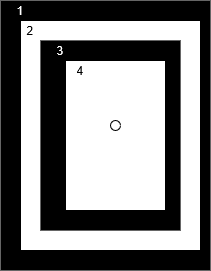
\includegraphics[width=3.2cm]{StadtInBundesland.png}
			\caption{Loch in einem Polygon in einem Loch von einem Polygon}
			\label{	StadtInBundesland}
		\end{center}
	\end{figure}\\
	\section{Ergebnisse}
	Die Flächen der einzelnen Bundesländer:\\
	\\
	\begin{tabular}{|c|c|}		
		\hline
		\textbf{Bundesland} & \textbf{Fläche}\\
		\hline
		Thüringen & 13725\\
		\hline
		Schleswig-Holstein & 13456\\
		\hline
		Sachsen-Anhalt & 17451\\
		\hline
		Sachsen & 15668\\
		\hline
		Saarland & 2180\\
		\hline
		Rheinland-Pfalz & 16914\\
		\hline
		Nordrhein-Westfalen & 28966\\
		\hline
		Niedersachsen & 40634\\
		\hline
		Mecklenburg-Vorpommern & 19659\\
		\hline
		Hessen & 17977\\
		\hline
		Hamburg & 633\\
		\hline
		Bremen & 341\\
		\hline
		Brandenburg & 25276\\
		\hline
		Berlin & 766\\
		\hline
		Bayern & 60026\\
		\hline
		Baden-Württemberg & 30522\\
		\hline
		Deutschland & 304194\\
		\hline
	\end{tabular}\\
	\vspace{2.0cm}\\
	Die Ergebnisse für die Städte die einzelnen Bundesländern zugewiesen werden:
	\vspace{0.5cm}\\
	\begin{tabular}{|c|c|}
		\hline
		\textbf{Bundesland} & \textbf{Landeshauptstadt}\\
		\hline
		Thüringen & Erfurt\\
		\hline
		Schleswig-Holstein & Kiel\\
		\hline
		Sachsen-Anhalt & Magdeburg\\
		\hline
		Sachsen & Dresden\\
		\hline
		Saarland & Saarbrücken\\
		\hline
		Rheinland-Pfalz & Mainz\\
		\hline
		Nordrhein-Westfalen & Düsseldorf\\
		\hline
		Niedersachsen & Hannover\\
		\hline
		Mecklenburg-Vorpommern & Schwerin\\
		\hline
		Hessen & Wiesbaden\\
		\hline
		Hamburg & Hamburg\\
		\hline
		Bremen & Bremen\\
		\hline
		Brandenburg & Potsdam\\
		\hline
		Berlin & Berlin\\
		\hline
		Bayern & München\\
		\hline
		Baden-Württemberg & Stuttgart\\
		\hline
	\end{tabular}
	
	
	\section{Testen des Algorithmus}
	Eine Möglichkeit ist es die Fläche mit der echten Daten aus Wikipedia zu vergleichen.\\
	\vspace{0.2cm}
	\scalebox{0.85}{
	\begin{tabular}{|c|c|c|c|}
		\hline
		\textbf{Bundesland} & \textbf{Algorithmus} & \textbf{Wikipedia} & \textbf{Faktor}\\
		\hline
		Thüringen & 13725 & 16202 & 0.8471 \\
		\hline
		Schleswig-Holstein & 13456 & 15800 & 0.8516 \\
		\hline
		Sachsen-Anhalt & 17451 & 20456 & 0.8530 \\
		\hline
		Sachsen & 15668 & 18449 & 0.8492 \\
		\hline
		Saarland & 2180 & 2571 & 0.8479 \\
		\hline
		Rheinland-Pfalz & 16914 & 19858 & 0.8517 \\
		\hline
		Nordrhein-Westfalen & 28966 & 34112 & 0.8491 \\
		\hline
		Niedersachsen & 40634 & 47709 & 0.8517 \\
		\hline
		Mecklenburg-Vorpommern & 19659 & 23295 & 0.8439 \\
		\hline
		Hessen & 17977 & 21115 & 0.8513\\
		\hline
		Hamburg & 633 & 755 & 0.8384 \\
		\hline
		Bremen & 341 & 419 & 0.8138\\
		\hline
		Brandenburg & 25273 & 29654 & 0.8522\\
		\hline
		Berlin & 768 & 891 & 0.8619 \\
		\hline
		Bayern & 60026 & 70541 & 0.8509\\
		\hline
		Baden-Württemberg & 30522 & 35747 & 0.8538\\
		\hline
		\hline
		Deutschland & 304194 & 357580 & 0.8507 \\
		\hline
	\end{tabular}
	}\\
	Im Grunde sich alle Verhältnisse sehr ähnlich. Ein grober Fehler ist erst einmal unwahrscheinlich. Diese Methode ist aber etwas zu ungenau um kleine Fehler zu entdecken. Dafür ist der Datensatz zu Fehlerhaft. So fehlen zum Beispiel einige innerdeutsche En- und Exklaven.\\
	Deshalb wurden über 50 Junit Tests geschrieben um die Funktionalität des Codes zu überprüfen. Diese Tests decken vorallem die bisher angesprochenen Randfälle ab. Die Tests wurden an Kommilitonen weitergegeben und diese bestätigten deren Qualität.\\
	Auch wurde jedes Bundesland genau untersucht. So wurde überprüft ob Inseln und Exklaven addiert werden und Löcher subtrahiert werden.\\
	Die korrekte Zuordnung der Landeshauptsädte
	
	
	\section{Komplexität}
	\begin{itemize}
		\item Die Komplexitätsklasse für das Einlesen der Daten liegt ist $\mathcal{O}(n)$, wobei n die Anzahl der Datenpunkte beschreibt.
		
		\item Die Komplexitätsklasse für das Berechnen der Fläche eines Polygon P ist $\mathcal{O}(n)$, wobei n die Anzahl der Eckpunkte des Polygons P beschreibt. Die oben durchgeführten Optimierungen verändern nichts an der Komplexitätsklasse sondern beschleunigen nur die Operationen selbst.
		
		\item Die Komplexitätsklasse für das Berechnen ob ein Punkt $\tilde{p}$ in einem Polygon P liegt ist $\mathcal{O}(n)$, wobei n die Anzahl der Eckpunkte des Polygons P beschreibt.
		
		\item Die Komplexitätsklasse für das Berechnen ob ein Polygon $P_1$ in einem Polygon $P_2$ liegt ist $\mathcal{O}(n^2)$. Dies entsteht da alle Kanten von $P_1$ mit allen Kanten von $P_2$ verglichen werden müssen. Dieser Vergleich alleine hat im Worstcase die Komplexität $\mathcal{O}(m*n)$  wobei m und n die Anzahl der Eckpunkte der Polygone $P_1$ und $P_2$ beschreibt. Zusätzlich muss noch getestet werden ob ein Punkte von $P_1$ in $P_2$ liegt was die Komplexität $\mathcal{O}(n)$ besitzt. Es muss nur ein Punkt getestet werden da schon überprüft wird ob sich die Kanten schneiden. Somit ist die Komplexität $\mathcal{O}(n^2+n)$ was trotzdem in der Komplexitätsklasse $\mathcal{O}(n^2)$ liegt.
		
		\item Die Komplexitätsklasse für das Berechnen wie viele Polygone aus einer Menge $\{P_1,P_2,...,P_n\}$ in einander liegen ist $\mathcal{O}(n^2)$, wobei n die Anzahl der Polygone beschreibt. Dies würde sich theoretisch optimieren lassen. Da aber die Menge der Polygone in der Aufgabe nie wirklich groß ist wäre der Aufwand für einer effizienteren Implementierung unverhältnismäßig groß und würde keine oder nur kleine Verbesserungen bringen.
	\end{itemize}
	Zusammengefasst kann man sagen das die je nach Aufgaben die Brechungen in der linearen oder in der quadratischen Komplexitätsklasse liegen.
	
	\begin{thebibliography}{00}
		\bibitem{b1}https://www.wikiwand.com/de/Gaußsche\_Trapezformel
		\bibitem{b2}http://www.dcs.gla.ac.uk/~pat/52233/slides/Geometry1x1.pdf
	\end{thebibliography}
	
	
	
	\section{Anhang}
	
	Berechnung der Fläche eines Polygons:
	

	\begin{lstlisting}[basicstyle=\tiny]
    /**
	* calculate the Area of this Polygon
	* @return double
	*/
	public double calculateArea(){
		if(!isClosed())
			throw new IllegalArgumentException("Polygon is not Closed");
		
		double area = 0;
		for(int counter = 1 ; counter < cords.size()-1; counter++)
			area += gausstriangle( cords.get(counter), cords.get(counter-1), cords.get(counter+1));
		
		area += gausstriangle( cords.get(0), cords.get(cords.size()-2), cords.get(1));
		return area/2;
	}
	
	
	private double gausstriangle(Point a, Point b, Point c){
		return a.getY()*(b.getX()-c.getX());
	}
	\end{lstlisting}
	
	Überprüfung ob Polygon $P_{this}$ in Polygon $P_{that}$ liegt:
	\begin{lstlisting}[basicstyle=\tiny]
/**
* Check if This is inside That
* @param that
* @return boolean
*/
public boolean isPolygonInside(Polygon that){
	if( !isClosed() || !that.isClosed() )
		throw new IllegalArgumentException("Polygon is not Closed");
	
	for(int thisCounter = 1; thisCounter < this.cords.size(); thisCounter++){
		final Line2Points thisLine = new Line2Points(this.cords.get(thisCounter-1), this.cords.get(thisCounter));
		for(int thatCounter = 1; thatCounter < that.cords.size(); thatCounter++){
			final Line2Points thatLine = new Line2Points(that.cords.get(thatCounter-1), that.cords.get(thatCounter));
			if(thisLine.isIntersecting(thatLine)){
				return false; // Is intersecting so this can not be in that
			}
		}
	}
	
	return that.isPointInside(this.getCords().get(0)); //check if one Point of this is in that   
}
	\end{lstlisting}
	Berechnung der Fläche eines Bundeslandes:
	\begin{lstlisting}[basicstyle=\tiny]
	public double calculateArea(){
		double sum = 0;
		for(Polygon p : areas){
			boolean isInside = false;
			for(Polygon p2 : areas){
				//Check if Hole
				if(!p.equals(p2) && p.isPolygonInside(p2) ){ 
					isInside = true;
					break;
				}   
			}
			if(isInside)
				sum -= Math.abs(p.calculateArea());
			else
				sum += Math.abs(p.calculateArea());
		}
		return sum;
	}
	\end{lstlisting}	
	
	Berechnung ob ein Punkt/Stadt in einem Bundeslandes liegt:
	\begin{lstlisting}[basicstyle=\tiny]
/**
* Polygone muessen vollstaendige Loecher voneinander sein. Sie duerfen sich nicht schneiden.
* @param p Punkt
* @return Ob Punkt in Polygon oder im Loch ist.
*/
public boolean isPointInside(Point p){
	final List<Polygon> relevantPolygons = areas.stream() 
	.filter(a -> a.isPointInside(p))
	.collect(Collectors.toList()); // all Polygons containing P
	
	
	return relevantPolygons.size()%2==1;
}
	\end{lstlisting}
	Berechnung ob ein Punkt in einem Polygon liegt:
\begin{lstlisting}[basicstyle=\tiny]
public boolean isPointInside(Point p){
	if(!isClosed())
		throw new IllegalArgumentException("Polygon is not Closed");
	//Check if Point lies on an edge
	final Line2Points pointLine = new Line2Points(p,p); // generate Dummy Line to check if it does intersect with Edges
	for(int counter = 1; counter < cords.size() ; counter++){
		if(pointLine.isIntersecting(new Line2Points(cords.get(counter-1),cords.get(counter)))) 
		return true;          
	}
	
	final double maxXValue = cords.stream()
		.mapToDouble(c -> c.getX())
		.reduce(Double::max)
		.orElseThrow(IllegalStateException::new);
	
	if(p.getX() > maxXValue)
		return false;
	
	final Point extreme = new Point(maxXValue+1, p.getY());
	
	int startCounter = 0;
	while(ccw(extreme, p, cords.get(startCounter)) == 0)
		startCounter++;
	
	int intersections = 0;
	double lr = orientation(extreme, p, cords.get(startCounter));
	for(int counter = startCounter+1; counter < cords.size() ; counter++){
		final double lrNew = orientation(extreme, p, cords.get(counter));
		if( Math.abs( lrNew - lr ) == 2){
			lr = lrNew;
			double o1 = ccw(cords.get(counter-1), cords.get(counter), extreme);
			double o2 = ccw(cords.get(counter-1), cords.get(counter), p);
			if(o1*o2<=0){
				intersections++;
			}
		}
	}
	for(int counter = 1; counter <= startCounter ; counter++){
		final double lrNew = orientation(extreme, p, cords.get(counter));
		if( Math.abs( lrNew - lr ) == 2){
			lr = lrNew;
			double o1 = ccw(cords.get(counter-1), cords.get(counter), extreme);
			double o2 = ccw(cords.get(counter-1), cords.get(counter), p);
			if(o1*o2<=0)
				intersections++;
		}
	}
	return intersections % 2 == 1; // return true if count is odd, false otherwise
}
\end{lstlisting}

	\end{document}
